%%%%%%%% ICML 2026 SENPAI SUBMISSION %%%%%%%%%%%%%%%%%

\documentclass{article}

\usepackage{microtype}
\usepackage{graphicx}
\usepackage{subcaption}
\usepackage{booktabs}
\usepackage{multirow}
\usepackage{array}
\usepackage{enumitem}
\usepackage{amsmath}
\usepackage{amssymb}
\usepackage{mathtools}
\usepackage{amsthm}
\usepackage{hyperref}
\usepackage[capitalize,noabbrev]{cleveref}

\newcommand{\theHalgorithm}{\arabic{algorithm}}

% Use preprint mode so author names render in the PDF.
% Preload bundled style dependencies so Tectonic does not substitute cached copies.
\usepackage{icml2026/algorithm}
\usepackage{icml2026/algorithmic}
\usepackage[preprint]{icml2026/icml2026}

\usepackage[disable,textsize=tiny]{todonotes}

\icmltitlerunning{SENPAI: An Observability-First Research Harness}

\begin{document}

\twocolumn[
  \icmltitle{SENPAI: Self-ExperimentatioN for Physical AI\\
  An Observability-First Research Harness}

  \icmlsetsymbol{equal}{*}

  \begin{icmlauthorlist}
    \icmlauthor{Thomas Capelle}{equal,wandb}
    \icmlauthor{Morgan McGuire}{equal,wandb}
    \icmlauthor{Justin Hodges}{coreweave}
  \end{icmlauthorlist}

  \icmlaffiliation{wandb}{Weights \& Biases, San Francisco, CA, USA}
  \icmlaffiliation{coreweave}{CoreWeave, Roseland, NJ, USA}
  \icmlcorrespondingauthor{Thomas Capelle}{tcapelle@wandb.com}
  \icmlcorrespondingauthor{Morgan McGuire}{morgan@wandb.com}
  \icmlcorrespondingauthor{Justin Hodges}{jhodges@coreweave.com}
  \icmlkeywords{Autonomous research, CFD surrogates, ML systems, agent observability, AI for science}

  \vskip 0.3in
]

\printAffiliationsAndNotice{\icmlEqualContribution}

\begin{abstract}
SENPAI (Self-Experimentation for Physical AI) is an observability-first research harness in which multi-agent state is grounded in pull requests and structured experiment logs rather than agent memory and scratchpads. Training CFD surrogates encompasses standard ML training considerations---architecture, optimizer, schedule, and loss design---but also physics-aware considerations such as boundary conditions, symmetries, and rollout stability. The harness orchestration is deliberately thin: an Advisor agent proposes hypotheses as GitHub pull requests; Student agents check out each PR, execute training based on the hypothesis, and write results back to the PR. Every hypothesis is grounded by a literature-search sub-agent callable by the Advisor or Student. A key contribution is observability-first memory and orchestration that goes beyond scratchpad files and in-context memory: SENPAI grounds state in the artifacts ML researchers already use---PRs, git history, and an experiment logger---producing an experiment ledger queryable by agents, researchers, and the harness itself. We run SENPAI on a Transolver model across TandemFoilSet, AirfRANS, and DrivAerML. On AirfRANS, the final recipe outperforms the reported Transolver baseline on surface-MSE; on TandemFoilSet, it is competitive with the normalized full-field MSE reported in the TandemFoilSet paper benchmark while also improving an internal balanced split; and on DrivAerML, preliminary runs approach secondary-provenance Transolver-family surface-pressure references. Taken together, the results show that AI scientists are most useful as near-autonomous co-workers that can run for long windows with minor course corrections. We release the harness, PR-indexed experiment ledger, and failure-mode analysis.
\end{abstract}

\section{Introduction}

Computational-fluid-dynamics (CFD) surrogates promise a practical acceleration layer for engineering design: inexpensive learned models can screen early-stage geometries, explore diverse operating regimes, and focus high-fidelity CFD or physical testing on later-stage decisions. Modern neural solvers now handle larger meshes, irregular geometries, tighter accuracy requirements, and smaller training sets than were feasible a few years ago \citep{zhou2026transolver3}. In principle, this makes hybrid workflows attractive, where learned surrogates complement established simulation pipelines.

In practice, adoption remains difficult for many small and mid-size engineering organizations. Training a useful CFD surrogate is not a routine application of standard ML: it requires decisions about architecture, optimization, normalization, boundary conditions, symmetries, rollout stability, and benchmark-specific evaluation \citep{wang2024cfdmlsurvey,hodges2024cfdmlmonograph}. The strongest models are typically produced by teams that combine ML expertise with domain knowledge in aerodynamics or fluid mechanics. Large enterprises can build such teams internally, but many engineering groups are constrained by safety-critical design processes, shortening development cycles, and expanding technical requirements. SENPAI targets this gap: it provides an autonomous research harness that can explore, document, and refine problem-specific surrogate recipes while keeping human engineers in the review loop.

Recent autonomous-research systems show that LLM agents can search literature, propose hypotheses, edit code, run experiments, and produce research reports. The AI Scientist generates ideas, implements experiments, writes papers, and runs automated review \citep{lu2024aiscientist,sakana2024aiscientist}; AI Scientist-v2 extends this with agentic tree search and workshop-level paper generation \citep{yamada2025aiscientistv2,sakana2025aiscientistv2}; Agent Laboratory structures literature review, experimentation, and report writing around a human-provided idea \citep{schmidgall2025agentlaboratory,schmidgall2025agentlaboratorycode}; and Jr. AI Scientist iteratively improves a baseline paper using modern coding agents \citep{miyai2026jraiscientist}. Other systems emphasize collaboration or external tooling: ResearchAgent generates and revises research ideas over scientific-literature graphs \citep{baek2024researchagent}, AgentRxiv lets agent laboratories upload and retrieve generated reports from a shared preprint server \citep{schmidgall2025agentrxiv}, ChemCrow and Coscientist connect LLM planners to chemistry tools and laboratory workflows \citep{bran2024chemcrow,boiko2023coscientist}, and FunSearch couples an LLM generator to a verifiable evaluator and scored program database \citep{romeraparedes2024funsearch}. These systems establish the value of tool use, execution, and persistent artifacts in autonomous research, but their state is typically organized as agent-owned files, generated papers, report stores, search populations, or conversation traces rather than as the ordinary audit trail of a multi-experiment ML research program.

The closest recent systems to SENPAI also recognize that long-horizon agents need to store state outside model context, but they store that state in different substrates. Kosmos maintains internal structured memory of literature-search and data-analysis summaries to choose later tasks \citep{mitchener2025kosmos}; AiScientist uses a permission-scoped File-as-Bus workspace so agents re-ground on file-based analyses, plans, code, logs, and experimental evidence \citep{chen2026aiscientist}; and grounded autonomous research externalizes state as rerunnable simulation artifacts within a single-paper reproduction loop \citep{huang2026groundedautonomousresearch}. SENPAI takes a complementary systems position: the authoritative state is the substrate human ML teams already inspect, namely pull requests for code review and discussion \citep{githubdocs_pullrequests}, git history for ordered code provenance \citep{chacon2014progit}, and an experiment tracker for metrics, hyperparameters, system metrics, checkpoints, and agent traces \citep{biewald2020wandb,wandbdocs_experiments}.

Long-running ML-engineering agents have also begun to appear outside the paper-generation setting. Hugging Face's \texttt{ml-intern} is an open-source agent that researches papers, writes ML code, launches training through the Hugging Face ecosystem, and maintains session history with auto-compaction and optional session upload \citep{huggingface2026mlintern}. Like AiScientist's File-as-Bus and AI Scientist-v2's tree and journal artifacts, this is durable agent state, but it is not a PR-indexed experiment ledger coupled to an experiment tracker. Reviewability depends on inspecting session traces or generated files rather than following the same pull-request, git-history, and W\&B substrate used by human ML teams.

SENPAI is deliberately thin. A new research-program branch is created; an Advisor reads the current experiment state from GitHub and W\&B, proposes a literature-grounded hypothesis as a pull request, and assigns it to one of $N$ GPU-backed Student agents. Each Student polls for its labeled PR, checks out the branch, modifies the training loop for the requested hypothesis, runs the experiment, and writes metrics, commands, W\&B links, and analysis back into the PR. The Advisor then merges the result, requests a revision, or closes the line of inquiry. Both roles can call a shared literature-search sub-agent. Humans remain in the loop through ordinary GitHub issues and PR comments. Scratchpad files are used as rough, noisy research logs, and the Advisor maintains a brief high-level research-state file, but ground-truth experiment state is externalized in PRs, git history, and W\&B runs. This queryable ground-truth state made the system more robust to drift in large scratchpad files, context compaction, restarts, and file loss, while leaving behind a durable experiment ledger as a by-product.

Over the course of the research programme, SENPAI created more than 2,700 pull requests and recorded more than 10,700 W\&B runs while deploying, at peak, 59 distinct Student agents.

\begin{table}[t]
  \caption{Scale of the SENPAI research program. Token counts are medians per pull request.}
  \label{tab:scale}
  \centering
  \small
  \begin{tabular}{@{}p{0.70\columnwidth}r@{}}
    \toprule
    Metric & Value \\
    \midrule
    Agent-generated PRs & 2,700+ \\
    PRs with at least one completed run & 2,300+ \\
    W\&B runs recorded & 10,700+ \\
    Peak concurrent Student agents & 59 \\
    Peak concurrent training runs & 347 \\
    Merged run-bearing PR latency, median & 48 min \\
    Merged run-bearing PR latency, p75 / p90 & 3.4 h / 6.6 h \\
    Median Student input tokens & 1,421,948 \\
    Median Student output tokens & 6,012 \\
    Median Advisor input tokens & 187,453 \\
    Median Advisor output tokens & 1,621 \\
    \bottomrule
  \end{tabular}
\end{table}

\textbf{Observability harness contribution.}
SENPAI contributes a new observability-first harness for semi-autonomous research. By grounding state in structured, queryable units of data---GitHub PRs, commits, and W\&B runs---we produce an experiment ledger that is both researcher- and agent-friendly. This structured logging enables the harness to reproducibly query past experiments, check the status of current experiments, identify idle resources, and expose successful and unsuccessful experiments to researchers through ordinary tools.

\textbf{Physical-AI contribution.}
SENPAI autonomously improves multiple CFD surrogate benchmarks starting from a basic Transolver model. Under the directly comparable aggregate AirfRANS full-regime surface-MSE protocol, SENPAI generated the lowest surface error we found (0.0030 best run; 0.0062 three-seed mean), although volume-MSE remains higher than the strongest reported volume results at 0.00764 versus 0.0017 for SpiderSolver \citep{qi2025spidersolver}. On DrivAerML, surface-pressure relative-$L_2$ reaches 4.62\% on validation and 6.24\% on test, improving the validation-side Transolver-family band while still trailing Transolver++, AB-UPT, and Transolver-3 \citep{alkin2025abupt,zhou2026transolver3}. On TandemFoilSet, SENPAI reaches normalized full-field test MSE near the paper's best Experiment-4 range on one preliminary paper-contract split, and reaches 24.58 denormalized surface-pressure MAE on the TandemFoilSet-Balanced parity contract \citep{lim2026tandemfoilset,mcguire2026tandemfoilsetbalanced}.

\textbf{Failure-mode taxonomy.}
SENPAI also contributes an empirical failure-mode analysis of long-running agentic ML research systems. Because every agent trajectory, tool call, PR transition, W\&B run, monitor event, and context compaction was logged, we can audit the system as an experimental object rather than describe failures anecdotally. We audit a 24-hour fleet trace containing 53,022 model requests and 5.24B tokens across one Advisor and 57 token-emitting Student agents. The dominant failure case was monitor-driven context bloat: 28,247 model-facing monitor events consumed 3.25B cache-inclusive tokens. Tool-use errors accounted for 892 of 25,365 tool uses (3.5\%), and routine Student coordination checks were a small part of total workload at 3.8\% of usage records. These measurements motivate bounded monitoring, durable external state, and executable handoff protocols more than additional prompt prose.

\section{Methodology: System Design}

State lives in pull requests and W\&B runs, not in agent memory or scratchpad files. Every other design choice follows from this constraint.

\begin{figure*}[t]
  \centering
  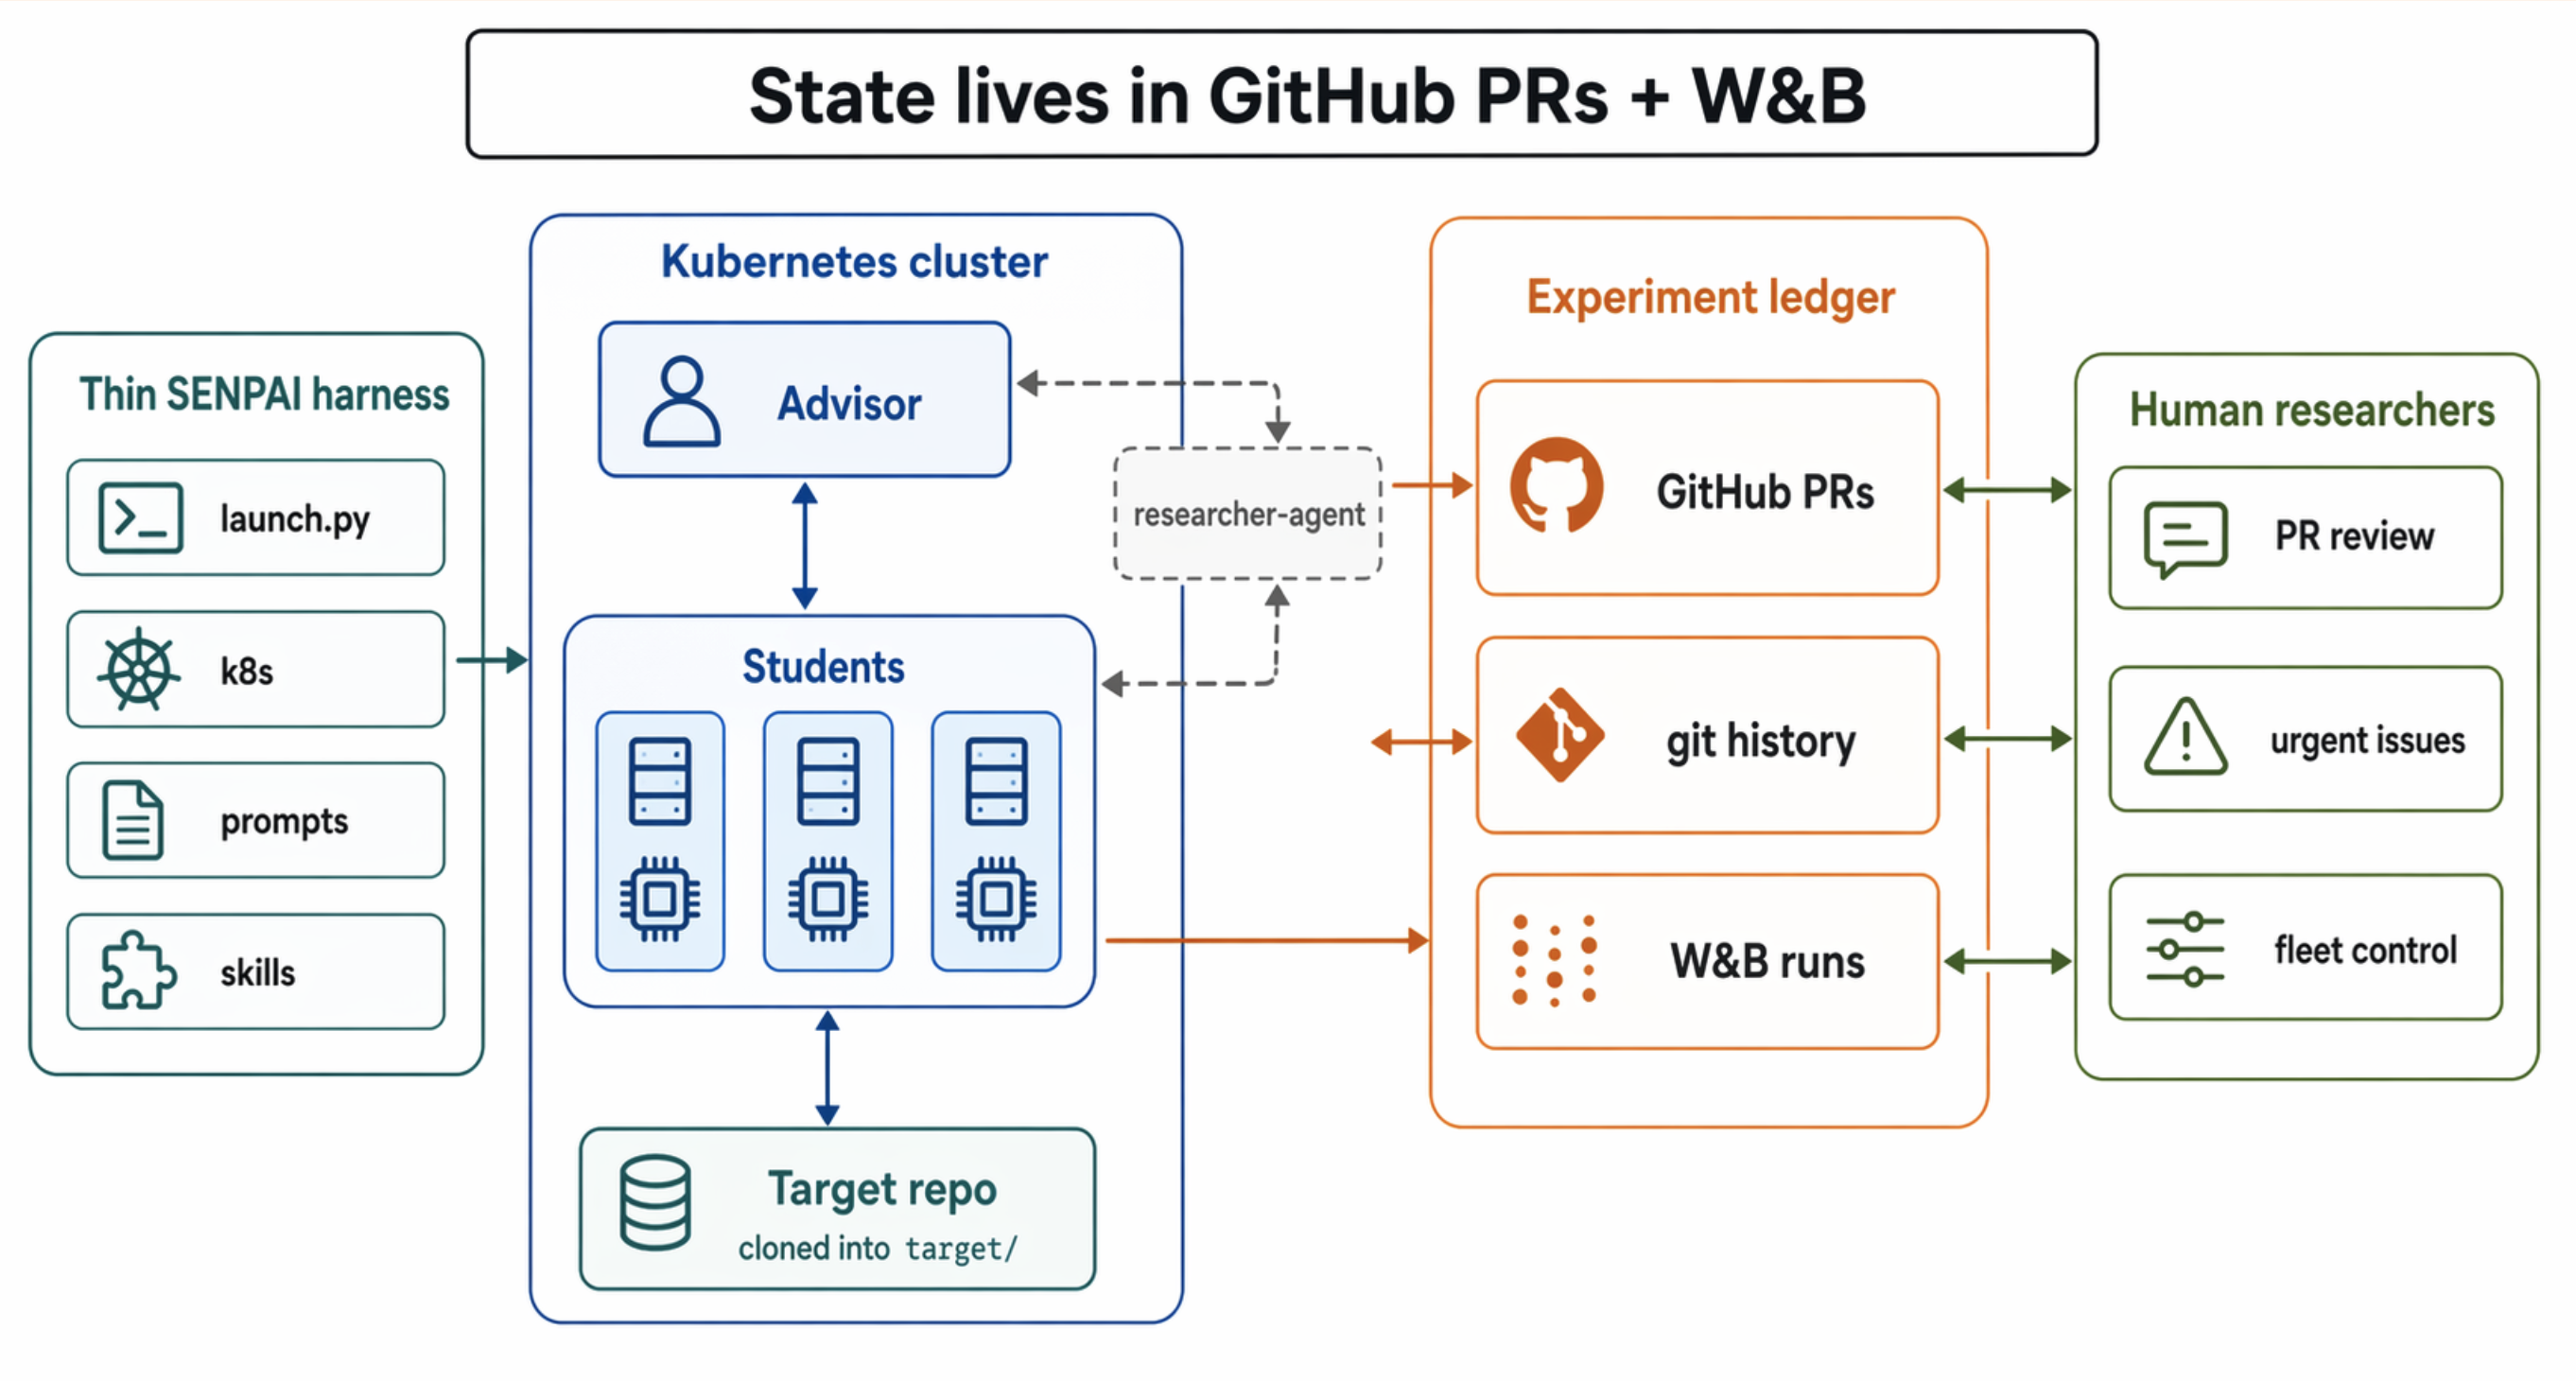
\includegraphics[width=0.78\textwidth]{section2_image.png}
  \caption{SENPAI deployment architecture. A thin harness deploys one Advisor and $N$ Student pods; both roles can call a shared researcher agent. Program state lives outside the cluster in the experiment ledger: GitHub PRs, git history, and W\&B runs.}
  \label{fig:architecture}
\end{figure*}

SENPAI organizes semi-autonomous CFD-surrogate research around artifacts human ML teams already produce---pull requests, git commits, and experiment-tracker runs---and two agent roles that read and write them (\cref{fig:architecture}). An Advisor runs a research sub-agent and proposes hypotheses by opening draft PRs; one of $N$ Students claims each PR, implements the hypothesis, runs training, and writes results back as PR comments linked to W\&B runs. A hypothesis's full trajectory---intent, metrics, and review---is therefore a standard GitHub PR log rather than an agent-internal trace. The rest of this section describes the research loop, the ledger, the harness loop, and the human-in-the-loop channels. Role prompts, the literature sub-agent design, the skill catalogue, and the Advisor's hypothesis-selection and merge rules are deferred to Appendix A.

\subsection{SENPAI's Research Loop}

Each experiment follows the same compact ledger-driven lifecycle:
\begin{description}[leftmargin=4.8em,labelwidth=4.3em,labelsep=0.5em,itemsep=0.15ex,topsep=0.5ex,parsep=0pt]
  \item[Research] Advisor decides whether to run the research sub-agent for the next batch of experiments.
  \item[Assign] Advisor drafts a PR with a hypothesis, exact training-code guidance, metrics to improve, and a Student label.
  \item[Run] Student polls for assigned PRs, checks out the PR branch, implements changes, and launches W\&B-logged training.
  \item[Report] Student posts experiment results, W\&B run ID, code changes, and analysis, then marks the PR ready for review.
  \item[Review] Advisor polls review-ready PRs and merges, requests follow-up work, or closes the inquiry.
  \item[Advance] If a PR is merged, Advisor updates the baseline against which subsequent PRs are compared.
\end{description}

\subsection{The Experiment Ledger: Pull Requests and Experiment Logger}

Every experiment is a pull request plus a set of W\&B logs. The PR body holds the hypothesis, experiment instructions, and baseline metrics to improve upon; the comment thread carries Student results and Advisor review notes. W\&B carries the quantitative side: each run documents the training config, result metric, scalar curves, system metrics, checkpoints, and, when enabled, agent traces. The two systems together form an observable experiment ledger: researcher-inspectable through familiar GitHub and W\&B interfaces, and machine-queryable through mature CLIs.

This design lowers the barrier for researchers to understand a system that can produce hundreds or thousands of experiments during a research program. Researchers can inspect an individual PR to understand the hypothesis and code diff, then open the associated W\&B run to inspect configs, curves, and checkpoints. Researchers' own agents can also query the same ledger to generate aggregate reports, detect stale branches, summarize failed lines of inquiry, and identify idle resources. Because the ledger is structured and external, pod restarts, context compactions, and fresh-container boots are less harmful: the next agent cycle can reconstruct the experiment state from PRs, git history, and W\&B rather than trusting local scratchpads.

In contrast to AgentRxiv \citep{schmidgall2025agentrxiv}, which shares papers between agents, SENPAI shares experiments within an existing code-review substrate. In addition to the core experiment ledger, the Advisor keeps a small set of focus-aid markdown files for research-state summaries, baseline tracking, experiment scratchpads, and dataset notes. These files are caches, not authoritative state. Earlier harness iterations treated them as durable, which produced silent drift when summaries disagreed with the ledger.

\subsection{SENPAI's Harness Loop}

SENPAI deploys as a small set of Kubernetes workloads: one Advisor CPU pod, $N$ Student GPU pods, and a shared persistent data volume for datasets and checkpoints. The harness image is stable across problems; a task repository is swapped in per programme, so every agent commit, branch, and PR lives in a self-contained target repository that a researcher can inspect independent of the harness.

The outer harness loop is a shell wrapper, not an LLM. The Advisor entrypoint wraps Claude Code in a loop inspired by Huntley's ``Ralph loop'' pattern. Programmatic triage determines whether Students are idle and whether new PRs, issues, or comments require attention, avoiding unnecessary LLM calls for polling. Later harness revisions encourage the coding agent to exit after handling actionable work; the outer loop resumes only when new information requires the session to continue.

\begin{figure*}[t]
\centering
{\setlength{\fboxsep}{2pt}%
\fbox{%
  \begin{minipage}{0.84\textwidth}
    \scriptsize
    \begin{algorithmic}[1]
      \STATE \texttt{iteration} $\gets 0$; \texttt{last\_check} $\gets \varnothing$
      \LOOP
        \STATE \texttt{iteration} $\gets$ \texttt{iteration} $+ 1$
        \STATE \texttt{review\_ready} $\gets$ \textsc{ListReviewReadyPRs}(\texttt{branch}, \texttt{last\_check})
        \STATE \texttt{human\_issues} $\gets$ \textsc{ListNewIssues}(\texttt{branch}, \texttt{last\_check})
        \STATE \texttt{idle\_students} $\gets$ \textsc{ListIdleStudents}(\texttt{student\_names}, \texttt{branch})
        \IF{\texttt{iteration} $> 1$ \AND \textsc{Empty}(\texttt{review\_ready}, \texttt{human\_issues}, \texttt{idle\_students})}
          \STATE \textsc{Sleep}(\texttt{tick}); \textbf{continue}
        \ENDIF
        \STATE \texttt{triage} $\gets$ \textsc{RenderTriage}(\texttt{review\_ready}, \texttt{human\_issues}, \texttt{idle\_students})
        \IF{\texttt{iteration} $= 1$}
          \STATE \texttt{exit\_code} $\gets$ \textsc{RunAgent}(\texttt{role\_prompt} $+$ \texttt{triage})
        \ELSE
          \STATE \texttt{exit\_code} $\gets$ \textsc{RunAgent}(\texttt{heartbeat} $+$ \texttt{triage}, \texttt{resume=true})
        \ENDIF
        \IF{\texttt{exit\_code} $= 0$}
          \STATE \texttt{last\_check} $\gets$ \textsc{MaxUpdatedAt}(\texttt{review\_ready}, \texttt{human\_issues})
        \ENDIF
        \STATE \textsc{Sleep}(\texttt{tick})
      \ENDLOOP
    \end{algorithmic}
  \end{minipage}%
}}
\caption{Simplified Advisor outer loop. Polling and triage happen outside the LLM; the agent is invoked only when there is actionable work.}
\label{fig:advisor-loop}
\end{figure*}

\subsection{Human-in-the-Loop}

Researchers can steer and interact with SENPAI through GitHub. The Advisor and Students poll GitHub issues regularly; this is the primary channel for asking questions of the Advisor or Students, or for providing a new research direction. This is deliberately low-bandwidth because SENPAI is designed to be semi-autonomous with infrequent guidance. Researchers can also comment on individual experiment PRs, although this was a less frequent interaction mechanism. During multi-day sessions, human actions were limited to research-direction corrections approximately once per day and pod restarts to release stuck Claude Code instances; no training-file or config edits were performed manually while the system was running.

\section{Experiments and Results}

\subsection{Experiment Setup}

Claude Code (v2.1.85 to v2.1.117) was run in headless mode as the agent harness for both the Advisor and Students. Claude Opus 4.6 drove early experimentation, while Claude Opus 4.7 drove later experiments. Advisor and Student instructions are reproduced in Appendix A. Student pods were scheduled on NVIDIA RTX 6000 Blackwell nodes with 96 GB VRAM per GPU and 8 GPUs per Student node. We tested up to $N=59$ concurrent Students, with peak concurrent training runs of 347. The harness experiments and iteration ran for one month, processing roughly 29 billion tokens.

\subsection{Data and Benchmarks}

To demonstrate SENPAI's CFD performance across multiple benchmarks, we train and evaluate on three CFD-surrogate datasets spanning 2D tandem-airfoil flow, 2D airfoil RANS, and 3D automotive aerodynamics: TandemFoilSet \citep{lim2026tandemfoilset}, AirfRANS \citep{bonnet2022airfrans}, and DrivAerML \citep{ashton2024drivaerml}.

\textbf{TandemFoilSet.} We use the paper's original Experiment 4 partition as one TandemFoilSet dataset and measure normalized full-field MSE. We generate a second split, TandemFoilSet-Balanced \citep{mcguire2026tandemfoilsetbalanced}, from \href{https://github.com/morganmcg1/tandemfoil2}{\texttt{morganmcg1/tandemfoil2}}, with 1,499 training cases and four balanced test splits: single-foil in-distribution, two unseen-front-camber geometry holdouts (race-car and cruise), and a Reynolds-number holdout. The average over these four splits is the primary parity metric, reported as denormalized surface-pressure MAE.

\textbf{AirfRANS.} We use the official full task with the last 10\% of the official training list held out for validation, giving a 720/80/200 train/validation/test split while keeping the official test set unchanged. We evaluate normalized targets on the official test split.

\textbf{DrivAerML.} We use the public surface split on the available processed cases, 400/34/50 train/validation/test, and measure surface-pressure relative-$L_2$ in percent, computed per case on unnormalized predictions and targets and then averaged over test cases.

\subsection{AirfRANS: Surface-MSE Below Published Transolver}

The official AirfRANS \texttt{full} task benchmark is defined on the pair of surface-MSE and volume-MSE evaluated on train-statistic-normalized targets \citep{bonnet2022airfrans}. Our best configuration achieves surface-MSE $=0.003$ (W\&B run \texttt{3e0ce368}, PR \#2824), an improvement over the strongest published surface reference in this comparison set, SpiderSolver at 0.0043 \citep{qi2025spidersolver}. Volume-MSE on the same run is 0.00764, roughly $4.5\times$ SpiderSolver's 0.0017. We therefore report a surface result competitive with published references and do not claim a full-benchmark win; closing the volume gap is open work.

Across three independent seeds (PR \#2831), surface-MSE was $0.00333 / 0.00668 / 0.00857$ (mean $0.0062$), and volume-MSE was $0.00886 / 0.00901 / 0.01709$ (mean $0.0117$). The best seed beats SpiderSolver on surface error; the mean seed does not. Seed-level volume remains above all published references in \cref{tab:airfrans}.

\begin{table}[t]
  \caption{AirfRANS full-task reference comparison. Metrics are train-statistic-normalized, per-case means on the official test split; lower is better.}
  \label{tab:airfrans}
  \centering
  \begin{tabular}{@{}lcc@{}}
    \toprule
    Method & Surf MSE & Vol MSE \\
    \midrule
    Transolver \citep{wu2024transolver} & 0.0142 & 0.0037 \\
    GeoANF \citep{li2024geoanf} & 0.0089 & 0.0062 \\
    SpiderSolver \citep{qi2025spidersolver} & 0.0043 & 0.0017 \\
    SENPAI, best run \texttt{3e0ce368} & \textbf{0.0030} & 0.00764 \\
    SENPAI, 3-seed mean & 0.0062 & 0.0117 \\
    \bottomrule
  \end{tabular}
\end{table}

The winning recipe was a 2-layer / 256-width / 4-head Transolver, AdamW with learning rate $7\cdot10^{-4}$, cosine schedule with $T_{\max}=5$, gradient clipping at 1.0, weight decay $10^{-2}$, EMA off, and Fourier positional features. The Advisor arrived at the 2-layer depth autonomously through a 4L/256d $\rightarrow$ 3L/256d ($-46.6\%$ surface-MSE) $\rightarrow$ 2L/256d ($-16.4\%$) sequence; wider 2-layer variants (384d, 512d) diverged early.

\subsection{TandemFoilSet: Two Benchmark Contracts, Reported Separately}

TandemFoilSet is evaluated in this paper under two distinct contracts: the paper-faithful Experiment 4 contract (normalized full-field MSE) and the packaged parity contract on the public \texttt{kagent} split family (denormalized surface-pressure MAE). They are not numerically interchangeable and we report them separately. Mixing the two under a single TandemFoilSet heading without relabeling the contracts would be scientifically misleading.

\subsubsection{TandemFoilSet Paper Contract: Preliminary}
Following the TandemFoilSet paper's Experiment 4 \citep{lim2026tandemfoilset}, we evaluate normalized full-field MSE (\texttt{field\_mse}) over the six task splits: \texttt{cruise\_random\_uniform}, \texttt{cruise\_random\_\{aoa,re,stagger,gap\}\_extrap}, and \texttt{racecar\_uniform}. The harness-released contract lives in \texttt{target/icml2026/tandemfoil\_paper/} with split-faithful train/test manifests; full provenance is in Appendix B.

At the time of writing, this lane remains immature. The best observed number is \texttt{test\_primary/field\_mse} $\approx 0.151$ on \texttt{cruise\_random\_uniform} on a non-converged development run, which sits between the paper-reported baseline ($1.79\pm1.38$) and best ($0.10\pm0.13$) on that task. We scope this benchmark as preliminary work and do not claim a competitive paper-contract result.

\subsubsection{TandemFoilSet Parity Contract (\texttt{kagent} Split): Harness-Driven Improvement}
The packaged parity target (\texttt{target/icml2026/tandemfoil/}) uses the public \texttt{kagent} v2 split: four balanced validation/test tracks (\texttt{single\_in\_dist}, \texttt{geom\_camber\_rc}, \texttt{geom\_camber\_cruise}, \texttt{re\_rand}). It reports denormalized pressure-channel surface MAE (\texttt{surface\_pressure\_mae}), aggregated globally over valid surface nodes. This is an internal SENPAI benchmark, not a literature comparator; we report it to quantify harness-driven improvement over SENPAI's own prior best.

Test surface-pressure MAE improved from 33.88 (run \texttt{v6amjkh7}, PR \#2810) to 24.58 (run \texttt{nrn0q3ct}, branch \texttt{robin/ema-warmup-tandem-0.999}), a 27\% reduction, entirely through PR-mediated Advisor--Student iteration with zero manual intervention between the two numbers. The pathway is visible in the PR ledger: early PRs stepped the learning rate down from $3\cdot10^{-4}$ to $1.25\cdot10^{-4}$ and added gradient clipping at 1.0; a subsequent EMA-warmup recipe family crossed the 25.0 MAE threshold.

\subsection{DrivAerML: Preliminary Surface-Pressure Transfer Result}

DrivAerML is treated as a transfer benchmark in this paper: we apply the shared Transolver stack used for AirfRANS and TandemFoilSet, evaluate on the public 400-train / 34-validation / 50-test split, and report mean per-case surface-pressure relative-$L_2$ on unnormalized predictions (\texttt{surface\_rel\_l2\_pct}). There is no single canonical public scalar in the DrivAerML literature, so we follow the AB-UPT and Transolver-3 reporting convention, which has converged on this metric, split family, and aggregation rule. We do not report a volume or multi-field comparison and scope this benchmark as surface-pressure transfer only, not a full multi-field result.

Our best-checkpoint numbers on the public split are validation $=4.62\%$ and test $=6.24\%$. The strongest directly comparable published references are Transolver-3 at 3.71\% and AB-UPT at 3.82\%. Our best-validation result sits in the secondary-provenance band for Transolver and Transolver++; our best-test result is above that band. We therefore report DrivAerML as preliminary transfer work and do not claim a competitive benchmark result.

\begin{table}[t]
  \caption{DrivAerML public-split surface-pressure relative-$L_2$ in percent. Metrics are mean per case on unnormalized predictions; lower is better.}
  \label{tab:drivaerml}
  \centering
  \small
  \begin{tabular}{@{}p{0.70\columnwidth}r@{}}
    \toprule
    Method & $p_s$ rel-$L_2$ (\%) \\
    \midrule
    Transolver-3 \citep{zhou2026transolver3} & 3.71 \\
    AB-UPT \citep{alkin2025abupt} & 3.82 \\
    Transolver++ (secondary) & 4.12 \\
    Transolver (secondary) & 4.81 \\
    SENPAI, best validation & 4.62 \\
    SENPAI, best test & 6.24 \\
    \bottomrule
  \end{tabular}
\end{table}

\paragraph{Deferred artifact figure.}
Figure 2, deferred to Appendix E, should reproduce a real SENPAI artifact: an anonymized PR conversation showing the Advisor hypothesis, Student result comment with best-checkpoint metrics, and Advisor merge decision, paired with a W\&B panel showing a surface-MSE curve annotated with PR-ledger events. This substantiates the paper's queryable-ledger claim.

\section{Discussion}

\subsection{What the PR+W\&B Grounding Bought Us}

\begin{itemize}[leftmargin=*]
  \item \textbf{Lossless session boundaries.} Crashed pods, context-limit compactions, and preempted Students all resumed by re-reading PR state on the next cycle.
  \item \textbf{Human-interruptible autonomy.} Reviewers steer the Advisor by commenting on PRs, not by editing prompts or restarting services.
  \item \textbf{Queryable retrospection.} The \texttt{list-experiments} workflow answered cross-benchmark questions, such as whether any prior run combined EMA warmup with gradient clipping on AirfRANS, directly against the ledger.
\end{itemize}

\subsection{Observable State as a Control Surface}

The PR and W\&B ledger made SENPAI useful as a research assistant rather than just an autonomous executor. By placing the core experiment ledger in systems already used by ML teams, the harness kept researchers close to the work without requiring them to supervise every experiment. Agents could run large numbers of experiments independently while researchers could still see, question, and redirect the broader research program through the tools they use daily.

This externalized state also reduced the fragility of this long-running system. When agents compacted, restarted, or lost local scratchpad context, the next cycle could reconstruct the experiment from the PR, git history, and W\&B runs.

Finally, the ledger turned a collection of individual experiments into a queryable research programme. Both researchers and agents could ask what had been tried, which failures were meaningful, which recipes transferred, and where progress had stalled. In this sense, SENPAI's core contribution is not replacing the researcher, but increasing the bandwidth at which researchers can understand, guide, and accelerate autonomous experimentation.

\subsection{\texttt{kagent}: Parallel Agents Under a Lighter Harness}

To contrast SENPAI's Advisor-mediated loop, we ran comparator cohorts under \texttt{kagent}, a lighter-weight harness that drops the Advisor/Student split and pull-request review logic in favor of a flat peer-competitive cohort and scoring-driven leaderboard. Each \texttt{kagent} agent runs a \emph{read-leaderboard $\rightarrow$ hypothesize $\rightarrow$ edit \texttt{train.py} $\rightarrow$ train $\rightarrow$ score $\rightarrow$ commit} loop with its own \texttt{EXPERIMENT\_JOURNAL.md} as durable memory. Agents see one another only through the shared leaderboard branch and public commits; there is no PR review, no merge gate, and no Advisor. We summarize the TandemFoilSet parity cohort here and defer the GRaM open-competition cohort to Appendix G.2. Every iteration, the agents start by consulting the public leaderboard and are prompted to be competitive:

\begin{quote}
{\footnotesize\itshape
Your objective is to top the leaderboard. If you are stuck with a low scoring solution, don't be afraid to try radical changes; marginal improvements on your low scoring solution are not going to cut it.
}
\end{quote}

\begin{table}[t]
  \caption{TandemFoilSet parity head-to-head over a 12-hour window. Lower MAE is better.}
  \label{tab:kagent-head-to-head}
  \centering
  \small
  \begin{tabular}{@{}p{0.38\columnwidth}ccc@{}}
    \toprule
    Harness & GPUs & Runs & MAE \\
    \midrule
    SENPAI, PR-mediated & $7 \times 8$ & 544 & 40.9 \\
    \texttt{kagent}, flat cohort & $8 \times 1$ & 223 & \textbf{34.41} \\
    \bottomrule
  \end{tabular}
\end{table}

On the same TandemFoilSet parity target, an eight-agent Opus 4.7 \texttt{kagent} cohort ran for 12 hours on the same dataset, split family, and primary metric as the SENPAI result in Section 3.2.2b. In that 12-hour head-to-head, \texttt{kagent} landed lower in absolute MAE, while SENPAI's multi-week PR-mediated anchor on the same benchmark remained lower at 24.58 MAE. The \texttt{kagent} winner scored 34.41 average surface-pressure MAE, a $3.5\times$ improvement over the Transolver starter. The decisive recipe---full-mesh training with small batch size, warm-started from a subsample-trained checkpoint---was independently rediscovered by three of the top four agents within a short window after leaderboard commits exposed it. The run artifacts are the \href{https://github.com/tcapelle/kagent/blob/6cfac55a619f3230a8549df3faabd058e2b402b6/leaderboard.md}{SHA-pinned leaderboard}, the \href{https://wandb.ai/wandb-applied-ai-team/kagent-tandemfoil}{W\&B project}, and the \href{https://github.com/tcapelle/kagent}{\texttt{tcapelle/kagent} repository}. The qualitative trade-off---review gating and indexed-into-the-ledger retrospection versus raw peer-diffusion speed---is the subject of Appendix G.1.

\subsection{Failure Modes: Where Long-Running Research Agents Break}

The recurring problems SENPAI encountered were harness-engineering problems---monitoring long-running jobs, recovering across compaction or restart, enforcing brittle tool interfaces, and keeping PR and W\&B state consistent---not primarily failures of experimental reasoning.

\textbf{Monitor-driven context bloat.} Students monitored training logs for progress, errors, checkpoint detection, and completion. Persistent log monitors caused small events to resume full long-lived agent sessions. In a 24-hour fleet trace, 615 Student monitor setups produced 28,247 model-facing monitor events and 28,246 direct model responses, consuming 3.25B cache-inclusive tokens. The median response reloaded roughly 110k cached tokens while adding only 347 uncached input tokens. Training logs should therefore be reduced by low-context processes that escalate only decision-relevant events: new-best checkpoints, milestones, errors, completion, or timeout.

\textbf{Tool-interface errors.} Tool-use errors accounted for 892 of 25,365 tool uses, or 3.5\%. The main causes were failed shell commands, GitHub scope errors, blocked wait patterns, wrong paths, failed pushes, oversized reads, and edit guards. A broader scan found 2,156 failure-like tool results, or 8.5\%, but many were training outcomes such as NaNs, out-of-memory failures, tracebacks, killed jobs, or divergent metrics. Failed runs can be scientific evidence if metrics and logs are captured; failed control actions require narrower, idempotent tool contracts.

\textbf{Compaction boundaries.} The trace contained 240 automatic compactions, with main Student contexts reduced from roughly 196k tokens to 3k-token continuation summaries. These summaries were sufficient for resumption but unsafe as ground truth. Decisions had to be revalidated against PR labels, PR comments, W\&B configuration, W\&B history, and live run state.

The ledger mitigated these failures. Among 39 Student sessions with final-like monitor signals, 38 had explicit PR-comment result evidence and 33 had ready or review-status handoff evidence. Even when sessions compacted, restarted, or delegated work, experiments usually survived as inspectable PR/W\&B artifacts.

The lesson is that long-running research agents need observable infrastructure more than additional prompt prose. Monitor bloat requires bounded observation; tool errors require executable helpers; training failures require mandatory result and checkpoint capture; state drift requires a single authoritative ledger, with summaries treated as caches. SENPAI did not eliminate failure, but it made failure measurable, attributable, and repairable.

\subsection{Limitations}

\begin{itemize}[leftmargin=*]
  \item Students operate on a shared \texttt{core/} library---architectures, datasets, features, optimizer, and metric contracts---plus a per-target \texttt{train.py} entry point. Students can modify these and frequently do, but \emph{de novo} architecture generation and cross-cutting refactors that would conflict with other live PRs remain out of scope.
  \item \emph{Near-autonomous} is literal: every result required an initial problem specification, a dataset, and downstream human PR review. Our unattended windows measure continuity between touchpoints, not unsupervised research.
  \item Reward hacking on surrogate metrics is mitigated but not eliminated by full-metric reporting (surface, volume, primary alias, and per-split breakdowns) and by ledger-level queryability.
  \item Compute and API costs were substantial; the released ledger makes future systems' per-merged-PR efficiency auditable.
  \item Results are not independently replicated at the time of writing.
  \item This paper was drafted with SENPAI-style AI assistance; all prose was reviewed and edited by the human authors in accordance with ICML 2026 LLM-use guidelines.
\end{itemize}

\section{Conclusion}

\textbf{Core claim.}
Grounding multi-agent research state with an observability focus via PRs and an experiment tracker---tools researchers already use---is sufficient to run a multi-week, semi-autonomous programme across CFD-surrogate benchmarks, with researchers intervening through ordinary PR review and a bounded issue channel.

\textbf{Hard-won design lessons.}
Tool misuse did not disappear under prompt hardening. Session mortality closed only through infrastructure fixes such as mandatory best-checkpoint saving. Derived summary state drifted silently from the authoritative ledger. Agentic research systems should be designed for these failure modes, not against them.

\textbf{Release commitment.}
We release the harness, PR-indexed experiment ledger, and failure-mode analysis as open-source artifacts.

\clearpage
\bibliographystyle{icml2026/icml2026}
\bibliography{paper}

\appendix

\section{Role Prompts, Sub-Agent, and Skill Catalogue}

\subsection{Role Prompts}

Advisor, Student, and \texttt{researcher-agent} prompt files are reproduced verbatim in the released repository and pinned to the versions used at the start of the sprint. They include the Advisor's hypothesis-selection and merge rules, plateau-escalation protocol, and the Student's result-comment schema.

\paragraph{Plateau protocol.}
When the Advisor observes five or more consecutive experiments with no improvement, it must escalate rather than stop:
\begin{enumerate}[leftmargin=*]
  \item \textbf{Change strategy tier.} If it has been tuning hyperparameters, move to architecture changes; if it has been on architecture, move to loss reformulation or data representation. Return to the literature and use the researcher-agent to find new ideas.
  \item \textbf{Revisit first principles.} Ask what the model fundamentally struggles with, inspect worst predictions, identify shared failure patterns, and anticipate skeptical reviewer objections.
  \item \textbf{Think bigger.} Look for techniques from fluid dynamics, numerical simulation, mathematics, physics, computer science, machine learning, or optimization that have not been tried.
  \item \textbf{Try bold ideas.} A plateau is permission to take bigger swings because conservative incremental experiments have been exhausted.
\end{enumerate}

\subsection{Skill Catalogue}

SENPAI's role prompts call a small catalogue of composable skills:
\begin{itemize}[leftmargin=*]
  \item \texttt{survey-prs}: Advisor-side read-only summary of review-ready, WIP, draft, and stalled PRs, plus idle Students.
  \item \texttt{poll-for-work}: Student-side read-only query for PRs carrying both \texttt{student:<name>} and \texttt{status:wip}.
  \item \texttt{check-human-issues}: Advisor- and Student-side issue channel for human messages tagged to the agent or team.
  \item \texttt{list-experiments}: paginated GraphQL scan of PRs that writes merged winners, compact result tables, and full PR bodies under \texttt{experiment\_log/}.
  \item \texttt{assign-experiment}: Advisor-side branch creation, push, draft PR creation, and label assignment.
  \item \texttt{submit-experiment-results}: Student-side commit, push, ready-for-review transition, and status-label swap.
  \item \texttt{merge-winner}: Advisor-side squash merge and baseline update, or conflict-driven send-back to the Student.
  \item \texttt{senpai-gh}: shared shell library for label swaps, send-back, close-with-comment, ready-for-review, and query primitives.
\end{itemize}

\section{Full Benchmark Result Tables}

\subsection{AirfRANS}

For paper-facing AirfRANS claims, the safe comparison contract is the official normalized-target surface-MSE plus volume-MSE on the official test split. A surface-only score is insufficient for a full AirfRANS benchmark win. The relevant comparator chain is Transolver, GeoANF, and SpiderSolver. The full appendix table should include AirfRANS frontier rows with surface and volume MSE plus W\&B run IDs.

\subsection{TandemFoilSet}

The original TandemFoilSet paper contract uses normalized full-field MSE over all valid nodes and channels. The packaged SENPAI parity contract uses denormalized surface-pressure MAE on a balanced \texttt{kagent} split family. These are both useful, but they answer different questions and should not be mixed in a single leaderboard. Full appendix tables should include TandemFoilSet parity progression by PR number and the sprint-populated paper-calibration row.

\subsection{DrivAerML}

The DrivAerML result is surface-first. The split and metric are comparable to AB-UPT and Transolver-3 for surface pressure, but SENPAI does not yet claim a full multi-field DrivAerML result. The full appendix table should include the DrivAerML validation/test trajectory.

\section{Failure-Mode Full Taxonomy}

\begin{table*}[h]
  \caption{Failure-mode taxonomy extracted from a 24-hour fleet trace.}
  \label{tab:failure-taxonomy}
  \centering
  \begin{tabular}{@{}p{0.22\textwidth}p{0.34\textwidth}p{0.34\textwidth}@{}}
    \toprule
    Category & Examples & Infrastructure response \\
    \midrule
    Monitor bloat & Log tails, checkpoint probes, repeated progress notifications entering full agent context & Low-context reducers; escalate only milestones, new-best checkpoints, terminal errors, completion, and timeout \\
    Tool contract failures & GitHub scope errors, wrong paths, blocked waits, failed pushes, oversized reads, missing branch preconditions & Narrow executable helpers; idempotent operations; explicit status transitions \\
    Training failures & NaNs, OOMs, killed jobs, divergent metrics, missing checkpoints & Treat as scientific evidence if metrics/logs are captured; require best-checkpoint save and PR comment \\
    State drift & Scratchpad summaries disagreeing with PR/W\&B state after compaction or restart & Treat summaries as caches; revalidate against PR labels, comments, W\&B configs, and run history \\
    \bottomrule
  \end{tabular}
\end{table*}

\section{Experiment Ledger Sample}

The released CSV schema records PR number, title, status, Student label, W\&B run IDs, primary metric name and value, baseline delta, era tag, merge-decision timestamp, and related metadata. This schema is intentionally close to the data already present in GitHub and W\&B so that no separate database is required for basic retrospection.

\section{Real SENPAI Artifact}

A redacted artifact figure should include a PR conversation on top and a W\&B panel on the bottom. The PR side should show the Advisor hypothesis body, Student result comment with best-checkpoint metrics, and Advisor merge decision. The W\&B side should show a metric curve annotated with PR-ledger events. This figure substantiates the abstract's queryable-ledger claim.

\section{Sprint Evidence Log}

The sprint evidence package consists of four artifact classes:
\begin{itemize}[leftmargin=*]
  \item \texttt{fetch\_experiments.py} snapshots at the beginning and end of the window, showing run-count deltas.
  \item Per-benchmark W\&B run panels from the window.
  \item \texttt{git log --oneline} on the Advisor branch, restricted to the sprint window.
  \item Two urgent-labeled GitHub issues with timestamps and Advisor actions.
\end{itemize}

\section{\texttt{kagent} Comparator Case Studies}

\subsection{TandemFoilSet Parity Run}

An eight-agent \texttt{kagent} cohort ran on the TandemFoilSet parity benchmark of Section 3.2.2b for roughly 12 hours without human intervention. The run used the same dataset, same public \texttt{kagent} v2 split family, and same primary metric: denormalized pressure-channel surface MAE averaged over \texttt{single\_in\_dist}, \texttt{geom\_camber\_rc}, \texttt{geom\_camber\_cruise}, and \texttt{re\_rand}. Each agent received a single GPU pod, a 30-minute-per-training-run budget, and the Transolver starter. Total activity was 330 agent commits and 223 scored leaderboard updates from the organiser.

Agents and organiser communicate through three channels only: a shared volume for data, predictions, and logs; the git remote for code and leaderboard state; and a \href{https://wandb.ai/wandb-applied-ai-team/kagent-tandemfoil}{W\&B project} for telemetry. There is no network path between agents, and each agent sees only its own competition-facing working directory. The organiser area holding ground truth and scoring code is invisible from inside an agent pod; scoring is the only privileged operation in the system.

\begin{table*}[h]
  \caption{Final \texttt{kagent} TandemFoilSet parity leaderboard. Lower is better.}
  \label{tab:kagent-final}
  \centering
  \begin{tabular}{@{}lrrrrr@{}}
    \toprule
    Agent & Avg surf-$p$ & Single in-dist & Geom RC & Geom cruise & Re rand \\
    \midrule
    frieren & \textbf{34.41} & 38.73 & 47.92 & 18.21 & 32.78 \\
    fern & 42.62 & 46.80 & 55.53 & 26.65 & 41.50 \\
    edward & 44.00 & 48.00 & 59.19 & 26.44 & 42.35 \\
    askeladd & 48.89 & 52.09 & 62.46 & 32.02 & 49.01 \\
    alphonse & 56.21 & 57.41 & 70.36 & 40.80 & 56.29 \\
    thorfinn & 62.57 & 45.81 & 77.35 & 40.44 & 86.70 \\
    tanjiro & 68.25 & 55.52 & 84.19 & 45.00 & 88.27 \\
    nezuko & 85.84 & 96.56 & 96.43 & 63.43 & 86.94 \\
    \bottomrule
  \end{tabular}
\end{table*}

The run proceeded in four phases: quick baselines, recipe convergence, warm-start fine-tune chains, and a full-mesh unlock. The defining finding was the subsampling trap: Transolver's slice-weight tensors are computed over the node population, so training on a 40k-point subsample while evaluating on roughly 240k nodes created a train/evaluation distribution gap. Three of the top four agents rediscovered this independently, with evidence in the commit-pinned journals for \href{https://github.com/tcapelle/kagent/blob/cdfa5d78e04aa2b6977e3d5ab8a8f4d1c0dfcc91/tandemfoil-competition/kaggler/EXPERIMENT_JOURNAL.md?plain=1#L39-L44}{Frieren}, \href{https://github.com/tcapelle/kagent/blob/d145d312660459324e386042eaa69a14f3a48d48/tandemfoil-competition/kaggler/EXPERIMENT_JOURNAL.md?plain=1#L72-L76}{Alphonse}, and \href{https://github.com/tcapelle/kagent/blob/a76f87a17574d9490d868edad359460f22a1465c/tandemfoil-competition/kaggler/EXPERIMENT_JOURNAL.md?plain=1#L32}{Edward}. Agents who did not try full-mesh fine-tuning generally stalled; the stalled reasoning is visible in the \href{https://github.com/tcapelle/kagent/blob/aa76905ad4467a95bcd914b588ef077802ce6c88/tandemfoil-competition/kaggler/EXPERIMENT_JOURNAL.md?plain=1#L37}{Thorfinn} and \href{https://github.com/tcapelle/kagent/blob/4e69f0371b01da656cd1dc89a3295cc0be50e3f9/tandemfoil-competition/kaggler/EXPERIMENT_JOURNAL.md?plain=1#L151}{Nezuko} journals.

Two secondary findings were robust. First, ensembles from the same warm-start lineage often regressed unless members were both strong and decorrelated; examples appear in the journals for \href{https://github.com/tcapelle/kagent/blob/d145d312660459324e386042eaa69a14f3a48d48/tandemfoil-competition/kaggler/EXPERIMENT_JOURNAL.md?plain=1#L110}{Alphonse}, \href{https://github.com/tcapelle/kagent/blob/054c788eb583dd052b87ca3a4dabcbcf75efa672/tandemfoil-competition/kaggler/EXPERIMENT_JOURNAL.md?plain=1#L125}{Askeladd}, and \href{https://github.com/tcapelle/kagent/blob/cdfa5d78e04aa2b6977e3d5ab8a8f4d1c0dfcc91/tandemfoil-competition/kaggler/EXPERIMENT_JOURNAL.md?plain=1#L99}{Frieren}. Second, the starter documentation's no-slip prior was misleading for this dataset: the surface mask included non-airfoil boundary nodes with non-zero velocity, and several agents disabled the constraint after inspecting data.

The scorer-race incident is a sibling failure mode to SENPAI's checkpoint-contract failures. \texttt{predict.py} writes the four \texttt{test\_*.pt} files sequentially; the organiser's scorer stamped commit directories with a missing file as \texttt{incomplete}, and the ``already scored'' check then treated \texttt{incomplete} as terminal even once all files were present. Every agent accumulated at least one incomplete entry; at least one agent diagnosed the bug and submitted a fresh commit hash instead of chasing the infrastructure issue. The infrastructure fix is to re-score incomplete entries whose files are now all present.

Core artifacts for this run are the \href{https://github.com/tcapelle/kagent/blob/apr23-leaderboard/leaderboard.md}{live leaderboard branch}, the \href{https://github.com/tcapelle/kagent/blob/6cfac55a619f3230a8549df3faabd058e2b402b6/leaderboard.md}{SHA-pinned leaderboard}, the \href{https://github.com/tcapelle/kagent/tree/apr23-leaderboard}{leaderboard tree}, the \href{https://github.com/tcapelle/kagent/tree/apr23/kaggler}{per-agent branches}, the \href{https://github.com/tcapelle/kagent/blob/cdfa5d78e04aa2b6977e3d5ab8a8f4d1c0dfcc91/tandemfoil-competition/kaggler/EXPERIMENT_JOURNAL.md}{winning Frieren journal}, and the \href{https://wandb.ai/wandb-applied-ai-team/kagent-tandemfoil}{W\&B project}.

\subsection{GRaM ICLR 2026 Open-Competition Run}

As a second comparator demonstration, sixteen Opus 4.6 agents were pointed at the \href{https://github.com/gram-competition/iclr-2026}{GRaM ICLR 2026 open competition}: predicting future 3D velocity fields around Formula-1 front-wing geometries for five future timesteps given five past, on roughly 100k-point meshes, scored by mean $L_2$ velocity error. The cohort ran for roughly 30 hours on 2026-03-29/30 with a single GPU per agent and a 30-minute per-training-run budget, starting from the reference MLP baseline. The \href{https://github.com/tcapelle/kagent/blob/20a631f83958a912e8ba1dcc0d7f372a99c2d3f4/leaderboard.md}{final leaderboard} showed a roughly $2\times$ spread across the cohort: winner \emph{violet} at 0.8526 $L_2$ against a roughly 1.75 reference-MLP baseline, \emph{gilbert} at 1.0230, \href{https://github.com/tcapelle/kagent/commit/e087be89ed601deda6770d25aefde9597409062b}{Thorfinn} at 1.0742, and \href{https://github.com/tcapelle/kagent/commit/731a5c0aafbb5635330c2e81a7cb17c82c368312}{Frieren} at 1.1535. Representative scored commits include \href{https://github.com/tcapelle/kagent/commit/9833cd308a}{Emma}, \href{https://github.com/tcapelle/kagent/commit/ac1af4d388}{Haku}, and \href{https://github.com/tcapelle/kagent/commit/89f15ea165}{Nezuko}. The strongest checkpoint was packaged and submitted upstream as \href{https://github.com/gram-competition/iclr-2026/pull/4}{PR \#4}, demonstrating a cold-start-to-external-submission pipeline in under two days. We report this run as a comparator, not as a benchmark claim. This run predates SENPAI's experiment-journal convention, so numeric claims resolve to the leaderboard commit and per-agent scored SHAs.

\end{document}
